\newpage
\setstretch{2}

%%%%%%%%%%%%%%%%%%%%%%%%%%%%%%%%%%%%%%%%%%%%%%%%%%%%%%%%%%%%%%%%%%%%%%%%%%%%%%%%%%%%%%%%%%%%%%%%%%%%%%%%%%%
%%%%%%%%%%%%%%%%%%%%%%%%%%%%%%%%%%%%%%%%%%%%%%%%%%%%%%%%%%%%%%%%%%%%%%%%%%%%%%%%%%%%%%%%%%%%%%%%%%%%%%%%%%%

%% Please enter the Chapter Title in the following in place of xxxxx. Use a label in place of yyyyy to be
%% referred later.
%% Please write the text in between the braces in place of AAAAA

%\chapter{Title of Chapter 01}
\chapter{introduction}
\label{ch1}

{Enter the material. The symbols and abbreviations defined can be used using the \textbackslash gls command. The defined symbol is \gls{mysymbol} and \gls{yoursymbol}. When the acronym is used for the first time it gives the full form as follows \gls{phd}. Thereafter, it only gives the abbreviation as follows \gls{phd}. The full form, short form and plural of the acronym can be called as follows \acrfull{phd}, \acrshort{phd} and \glspl{phd} respectively.

%%%%%%%%%%%%%%%%%%%%%%%%%%%%%%%%%%%%%%%%%%%%%%%%%%%%%%%%%%%%%%%%%%%%%%%%%%%%%%%%%%%%%%%%%%%%%%%%%%%%%%%%%%%

%% Please enter the Section Title in the following in place of xxxxx. Use a label in place of yyyyy to be
%% referred later.
%% Please write the text in between the braces in place of AAAAA

%\section{$1^{st}$ Section Title}
\section{Overview and Motivation}
\label{sec1.1}

\begin{comment}
{Typically the first chapter is the Introduction. The main goal of your introduction is to identify a problem that is worthy of investigation. It must also provide some idea of your research goals and approach to research.  Specific objectives can be introduced in the introduction chapter or they can be saved for later after you've provided additional background on the topic and state of the current research and its gaps.  The Introductory chapter often concludes with a summary of the organization of the thesis, including identification of the general content of specific chapters and appendices.}
\end{comment}

%%%%%%%%%%%%%%%%%%%%%%%%%%%%%%%%%%%%%%%%%%%%%%%%%%%%%%%%%%%%%%%%%%%%%%%%%%%%%%%%%%%%%%%%%%%%%%%%%%%%%%%%%%%

%% Please enter the Section Title in the following in place of xxxxx. Use a label in place of yyyyy to be
%% referred later.
%% Please write the text in between the braces in place of AAAAA

%\section{$2^{nd}$ Section Title}
\section{Problem Statement}
\label{sec1.2}

\begin{comment}
{Ideally, chapter one defines the overall importance of the problem areas and provides an introduction into what you did, chapter two is why you did it in the context of what was previously known, three is how you did it, four is what you found and five is what it all means - putting the pieces together, (what's your contribution to the research field).
%It should be noted that the objectives of your research define the OUTCOME, i.e. what will be learned.}
\end{comment}

%% Sub-Sections are used if / where necessary.
%% Please enter the Sub-Section Title in the following in place of xxxxx. Use a label in place of yyyyy to
%% be referred later.
%% Please write the text in between the braces in place of AAAAA

\section{Dissertation Organization}
\label{sec1.3}

\subsection{Sub-Section Title}
\label{}

{The Section has the $2^{nd}$ order heading. Enter subject matter for Sub-Section.}

%% Use the following snippet to insert the figure. Enter the file name with extension in place of xxxx

\begin{figure}[htb]
\centering
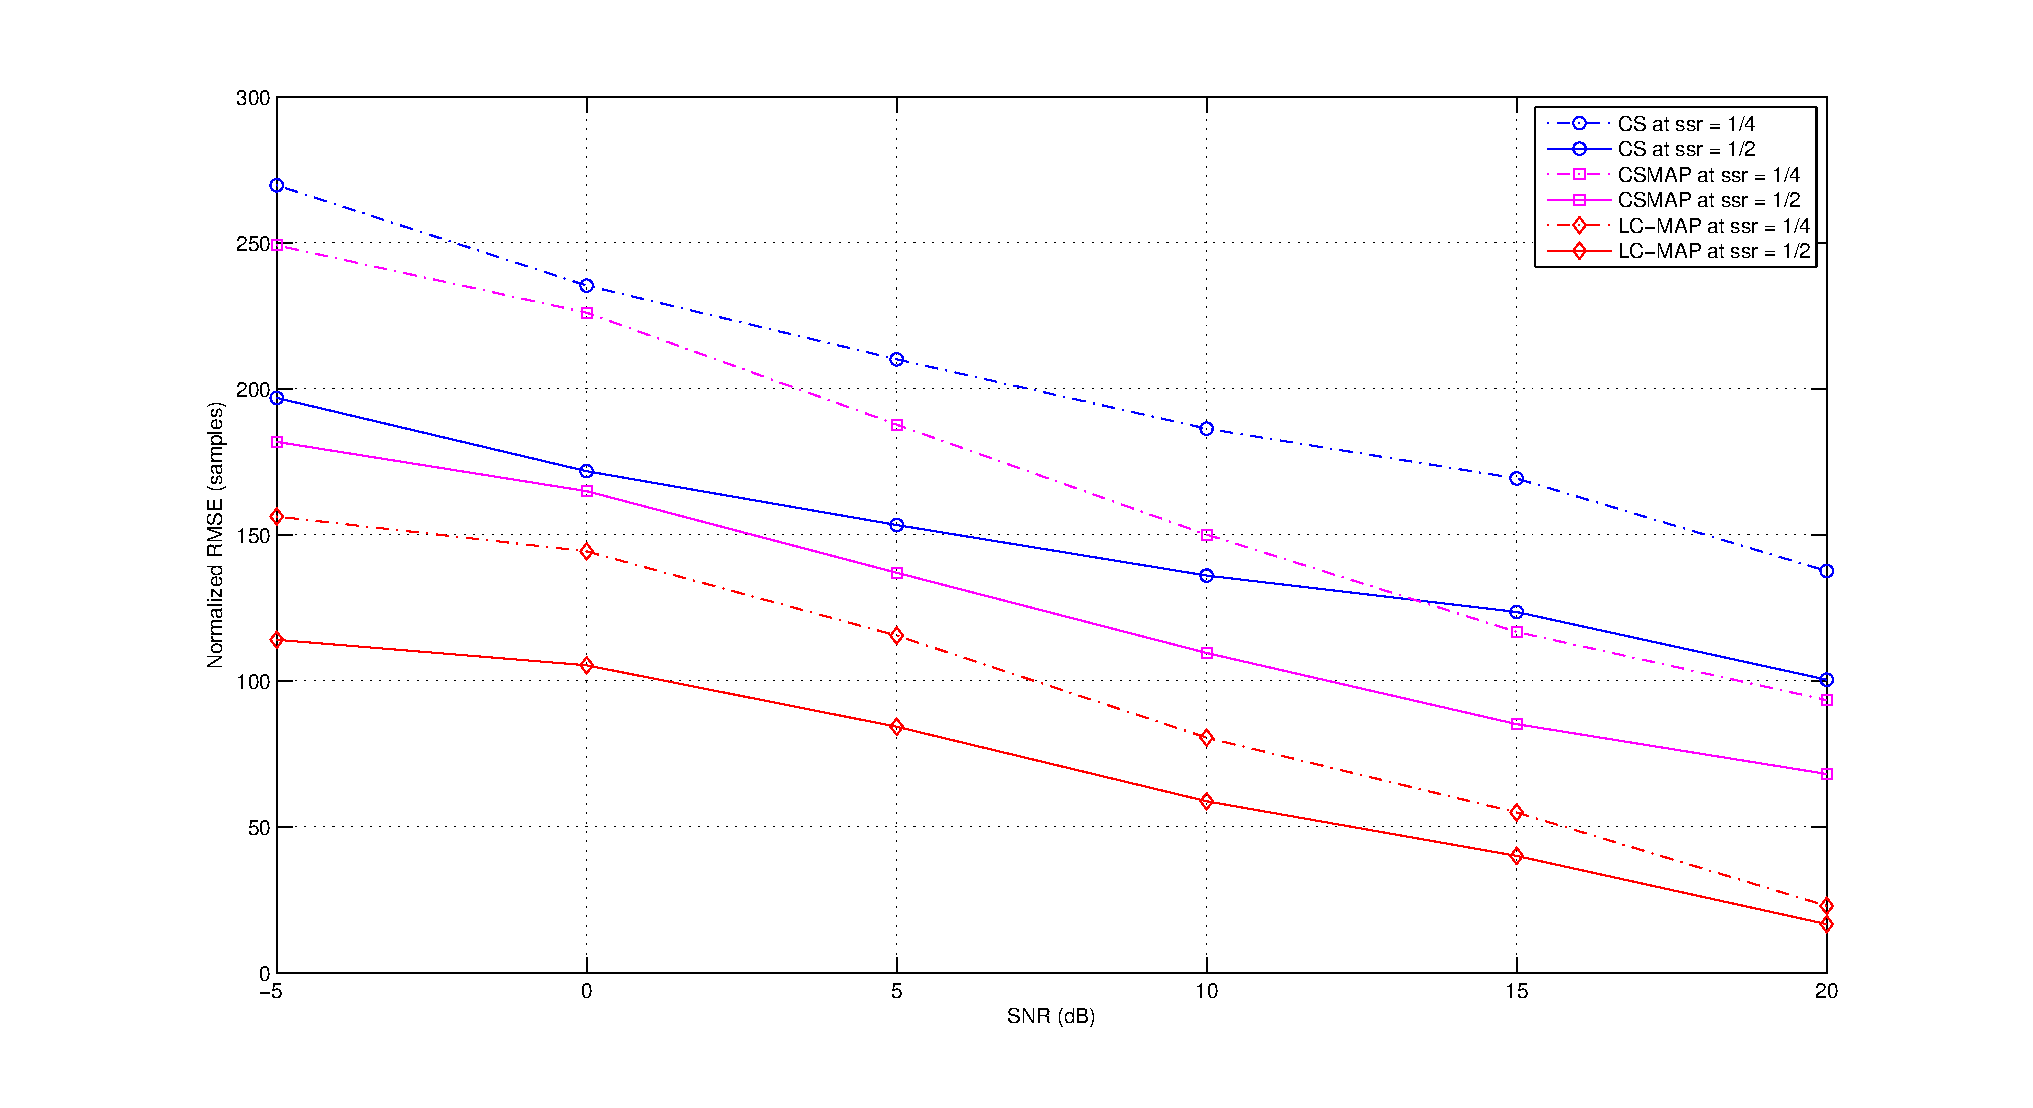
\includegraphics[width= 7.5cm, height= 5.26cm]{plot.eps}
\caption{This is a plot to show the results.}
\label{fig:Plot}
\end{figure}

%% Sub-Sub-Sections are used if / where necessary.
%% Please enter the Sub-Sub-Section Title in the following in place of xxxxx. Use a label in place of yyyyy
%% to be referred later.
%% Please write the text in between the braces in place of AAAAA

\subsection{Sub-Section Title}
\label{}

{The Section has the $2^{nd}$ order heading. Enter subject matter for Sub-Section.}

\begin{table}[h]
\centering
\begin{tabular}{|c|c|c|c|c|c|c|}
\hline
Itr. No. & $\boldsymbol \Theta_n$ & Size of $\underline{\boldsymbol \alpha}_i$ & \multicolumn{4}{c|}{Residual: $r_i^n = \Vert \mathbf{y} \Vert_{\boldsymbol \Sigma_i}^{2}$ }\\ \cline{4-7}
$(n)$ & $(L \times n)$ & $(n \times 1)$ &
$i=1$ & $i=2$ & \dots \dots & $i=C$ \\
\hline
1 & $\boldsymbol \Theta_1 = [\boldsymbol \theta_1]$ & $(1 \times 1)$ & $r_1^1$
& $r_2^1$
& \dots \dots & $r_C^1$ \\
\hline
2 & $\boldsymbol \Theta_2 = [\boldsymbol \Theta_1 \boldsymbol \theta_2]$ & $(2 \times 1)$ &  $r_1^2$ & $r_2^2$
& \dots \dots & $r_C^2$  \\
\hline
3 & $\boldsymbol \Theta_3 = [\boldsymbol \Theta_2 {\boldsymbol \theta_3}]$ & $(3 \times 1)$ & $r_1^3$ & $r_2^3$
& \dots \dots & $r_C^3$  \\
\hline
\vdots & \vdots & \vdots & \vdots & \vdots & \dots \dots & \vdots \\
\vdots & \vdots & \vdots & \vdots & \vdots & \dots \dots & \vdots \\
\hline
$L-1$ & $\boldsymbol \Theta_{L-1} = [\boldsymbol \Theta_{L-2} {\boldsymbol \theta_{L-1}}]$ & $((L-1) \times 1)$ & $r_1^{L-1}$ & $r_2^{L-1}$
& \dots \dots & $r_C^{L-1}$\\
\hline
$L$ & $\boldsymbol \Theta_L = [\boldsymbol \Theta_{L-1} {\boldsymbol \theta_{L-1}}]$ & $(L \times 1)$ &  $r_1^L$ & $r_2^L$
& \dots \dots & $r_C^L$  \\
\hline
\end{tabular}
\caption{This is a Table.}
\label{tab:Table}
\end{table}

%%%%%%%%%%%%%%%%%%%%%%%%%%%%%%%%%%%%%%%%%%%%%%%%%%%%%%%%%%%%%%%%%%%%%%%%%%%%%%%%%%%%%%%%%%%%%%%%%%%%%%%%%%%

%% Please enter the Section Title in the following in place of xxxxx. Use a label in place of yyyyy to be
%% referred later.
%% Please write the text in between the braces in place of AAAAA

\section{$3^{rd}$ Section Title}
\label{}

{Enter the section material.}

%%%%%%%%%%%%%%%%%%%%%%%%%%%%%%%%%%%%%%%%%%%%%%%%%%%%%%%%%%%%%%%%%%%%%%%%%%%%%%%%%%%%%%%%%%%%%%%%%%%%%%%%%%%

%% Please enter the Section Title in the following in place of xxxxx. Use a label in place of yyyyy to be
%% referred later.
%% Please write the text in between the braces in place of AAAAA

\section{$4^{th}$ Section Title}
\label{}

{Enter the section material.}

%%%%%%%%%%%%%%%%%%%%%%%%%%%%%%%%%%%%%%%%%%%%%%%%%%%%%%%%%%%%%%%%%%%%%%%%%%%%%%%%%%%%%%%%%%%%%%%%%%%%%%%%%%%
